\question \textbf{Title}

\begin{parts}
\part Given the same bitvector $B$ and the solution for $S$ from task 2, Write down the helper data structure $V$ and $I$ to support select operations in $O(\log \log n)$. When deciding whether a block is long or short, go by the definition from the lecture.


\begin{solution}

    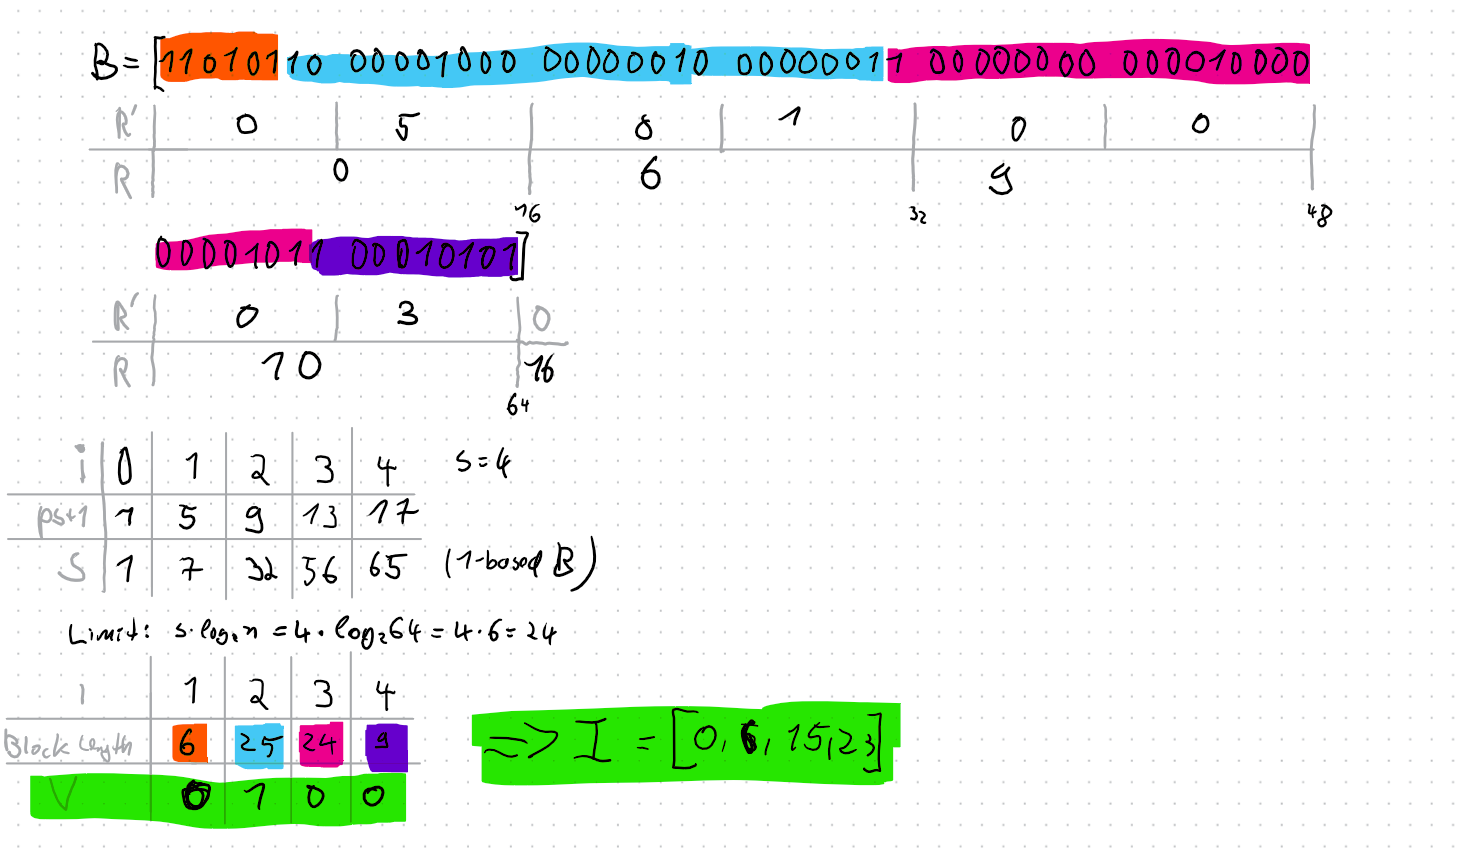
\includegraphics[width=\linewidth]{task_3/a6_a31.png}
\end{solution}


\part Compute $\text{select}(B, 6)$ again using your solution for $S$, $V$ and $I$ from above (Note that while $S$ is 0-based, $V$ and $I$ are 1-based).
\begin{solution}

    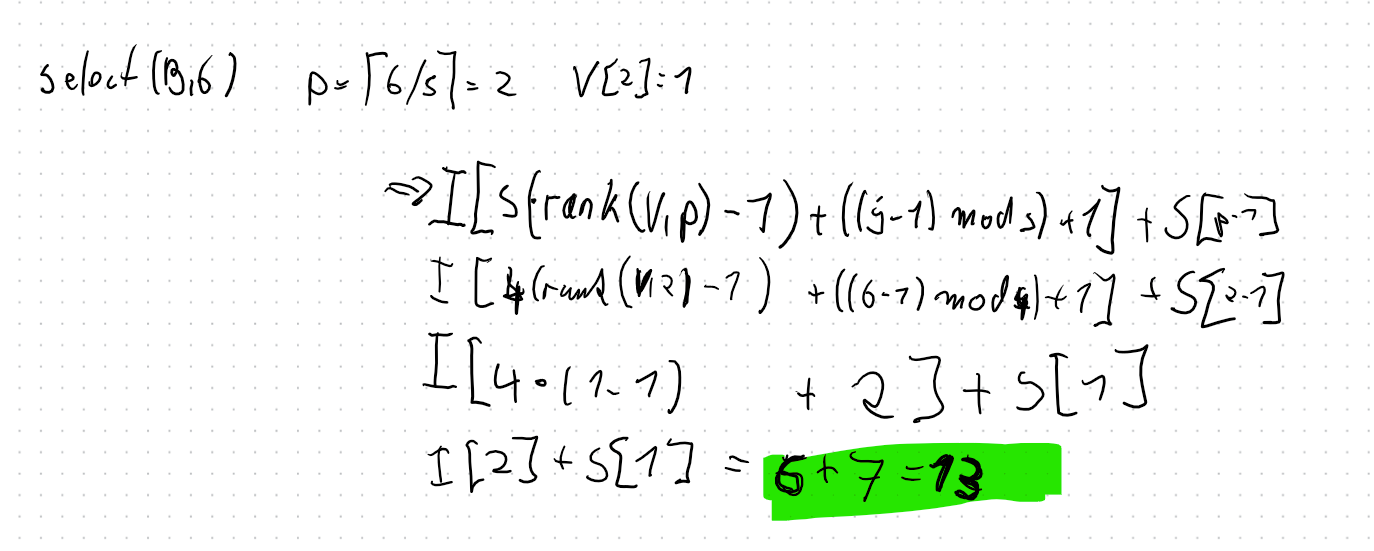
\includegraphics[width=\linewidth]{task_3/a6_a32.png}
\end{solution}

\end{parts}


% For tasks without simply remove the \begin{parts}...\part...\end{parts} commands